% Options for packages loaded elsewhere
\PassOptionsToPackage{unicode}{hyperref}
\PassOptionsToPackage{hyphens}{url}
%
\documentclass[
  english,
  man,floatsintext]{apa6}
\title{Assessing test-retest reliability of the infant preference measures}
\author{Melanie S. Schreiner\textsuperscript{1,2} \& the ManyBabies Test-Retest Consortium\textsuperscript{}}
\date{}

\usepackage{amsmath,amssymb}
\usepackage{lmodern}
\usepackage{iftex}
\ifPDFTeX
  \usepackage[T1]{fontenc}
  \usepackage[utf8]{inputenc}
  \usepackage{textcomp} % provide euro and other symbols
\else % if luatex or xetex
  \usepackage{unicode-math}
  \defaultfontfeatures{Scale=MatchLowercase}
  \defaultfontfeatures[\rmfamily]{Ligatures=TeX,Scale=1}
\fi
% Use upquote if available, for straight quotes in verbatim environments
\IfFileExists{upquote.sty}{\usepackage{upquote}}{}
\IfFileExists{microtype.sty}{% use microtype if available
  \usepackage[]{microtype}
  \UseMicrotypeSet[protrusion]{basicmath} % disable protrusion for tt fonts
}{}
\makeatletter
\@ifundefined{KOMAClassName}{% if non-KOMA class
  \IfFileExists{parskip.sty}{%
    \usepackage{parskip}
  }{% else
    \setlength{\parindent}{0pt}
    \setlength{\parskip}{6pt plus 2pt minus 1pt}}
}{% if KOMA class
  \KOMAoptions{parskip=half}}
\makeatother
\usepackage{xcolor}
\IfFileExists{xurl.sty}{\usepackage{xurl}}{} % add URL line breaks if available
\IfFileExists{bookmark.sty}{\usepackage{bookmark}}{\usepackage{hyperref}}
\hypersetup{
  pdftitle={Assessing test-retest reliability of the infant preference measures},
  pdfauthor={Melanie S. Schreiner1,2 \& the ManyBabies Test-Retest Consortium},
  pdflang={en-EN},
  pdfkeywords={language acquisition; speech perception; infant-directed speech; adult-directed speech, test-retest reliability},
  hidelinks,
  pdfcreator={LaTeX via pandoc}}
\urlstyle{same} % disable monospaced font for URLs
\usepackage{graphicx}
\makeatletter
\def\maxwidth{\ifdim\Gin@nat@width>\linewidth\linewidth\else\Gin@nat@width\fi}
\def\maxheight{\ifdim\Gin@nat@height>\textheight\textheight\else\Gin@nat@height\fi}
\makeatother
% Scale images if necessary, so that they will not overflow the page
% margins by default, and it is still possible to overwrite the defaults
% using explicit options in \includegraphics[width, height, ...]{}
\setkeys{Gin}{width=\maxwidth,height=\maxheight,keepaspectratio}
% Set default figure placement to htbp
\makeatletter
\def\fps@figure{htbp}
\makeatother
\setlength{\emergencystretch}{3em} % prevent overfull lines
\providecommand{\tightlist}{%
  \setlength{\itemsep}{0pt}\setlength{\parskip}{0pt}}
\setcounter{secnumdepth}{-\maxdimen} % remove section numbering
% Make \paragraph and \subparagraph free-standing
\ifx\paragraph\undefined\else
  \let\oldparagraph\paragraph
  \renewcommand{\paragraph}[1]{\oldparagraph{#1}\mbox{}}
\fi
\ifx\subparagraph\undefined\else
  \let\oldsubparagraph\subparagraph
  \renewcommand{\subparagraph}[1]{\oldsubparagraph{#1}\mbox{}}
\fi
\newlength{\cslhangindent}
\setlength{\cslhangindent}{1.5em}
\newlength{\csllabelwidth}
\setlength{\csllabelwidth}{3em}
\newlength{\cslentryspacingunit} % times entry-spacing
\setlength{\cslentryspacingunit}{\parskip}
\newenvironment{CSLReferences}[2] % #1 hanging-ident, #2 entry spacing
 {% don't indent paragraphs
  \setlength{\parindent}{0pt}
  % turn on hanging indent if param 1 is 1
  \ifodd #1
  \let\oldpar\par
  \def\par{\hangindent=\cslhangindent\oldpar}
  \fi
  % set entry spacing
  \setlength{\parskip}{#2\cslentryspacingunit}
 }%
 {}
\usepackage{calc}
\newcommand{\CSLBlock}[1]{#1\hfill\break}
\newcommand{\CSLLeftMargin}[1]{\parbox[t]{\csllabelwidth}{#1}}
\newcommand{\CSLRightInline}[1]{\parbox[t]{\linewidth - \csllabelwidth}{#1}\break}
\newcommand{\CSLIndent}[1]{\hspace{\cslhangindent}#1}
% Manuscript styling
\usepackage{upgreek}
\captionsetup{font=singlespacing,justification=justified}

% Table formatting
\usepackage{longtable}
\usepackage{lscape}
% \usepackage[counterclockwise]{rotating}   % Landscape page setup for large tables
\usepackage{multirow}		% Table styling
\usepackage{tabularx}		% Control Column width
\usepackage[flushleft]{threeparttable}	% Allows for three part tables with a specified notes section
\usepackage{threeparttablex}            % Lets threeparttable work with longtable

% Create new environments so endfloat can handle them
% \newenvironment{ltable}
%   {\begin{landscape}\centering\begin{threeparttable}}
%   {\end{threeparttable}\end{landscape}}
\newenvironment{lltable}{\begin{landscape}\centering\begin{ThreePartTable}}{\end{ThreePartTable}\end{landscape}}

% Enables adjusting longtable caption width to table width
% Solution found at http://golatex.de/longtable-mit-caption-so-breit-wie-die-tabelle-t15767.html
\makeatletter
\newcommand\LastLTentrywidth{1em}
\newlength\longtablewidth
\setlength{\longtablewidth}{1in}
\newcommand{\getlongtablewidth}{\begingroup \ifcsname LT@\roman{LT@tables}\endcsname \global\longtablewidth=0pt \renewcommand{\LT@entry}[2]{\global\advance\longtablewidth by ##2\relax\gdef\LastLTentrywidth{##2}}\@nameuse{LT@\roman{LT@tables}} \fi \endgroup}

% \setlength{\parindent}{0.5in}
% \setlength{\parskip}{0pt plus 0pt minus 0pt}

% \usepackage{etoolbox}
\makeatletter
\patchcmd{\HyOrg@maketitle}
  {\section{\normalfont\normalsize\abstractname}}
  {\section*{\normalfont\normalsize\abstractname}}
  {}{\typeout{Failed to patch abstract.}}
\patchcmd{\HyOrg@maketitle}
  {\section{\protect\normalfont{\@title}}}
  {\section*{\protect\normalfont{\@title}}}
  {}{\typeout{Failed to patch title.}}
\makeatother
\shorttitle{test-retest reliability of the infant preference measures}
\keywords{language acquisition; speech perception; infant-directed speech; adult-directed speech, test-retest reliability\newline\indent Word count: 3070}
\DeclareDelayedFloatFlavor{ThreePartTable}{table}
\DeclareDelayedFloatFlavor{lltable}{table}
\DeclareDelayedFloatFlavor*{longtable}{table}
\makeatletter
\renewcommand{\efloat@iwrite}[1]{\immediate\expandafter\protected@write\csname efloat@post#1\endcsname{}}
\makeatother
\usepackage{lineno}

\linenumbers
\usepackage{csquotes}
\ifXeTeX
  % Load polyglossia as late as possible: uses bidi with RTL langages (e.g. Hebrew, Arabic)
  \usepackage{polyglossia}
  \setmainlanguage[]{english}
\else
  \usepackage[main=english]{babel}
% get rid of language-specific shorthands (see #6817):
\let\LanguageShortHands\languageshorthands
\def\languageshorthands#1{}
\fi
\ifLuaTeX
  \usepackage{selnolig}  % disable illegal ligatures
\fi


\affiliation{\vspace{0.5cm}\textsuperscript{1} University of Goettingen\\\textsuperscript{2} Leibniz Science Campus PrimateCognition}

\abstract{
The ManyBabies1 collaborative research project (hereafter, MB1; Frank et al., 2017; ManyBabies Consortium, 2020) explores the reproducibility of the well-studied and robust phenomenon of infants' preference of infant-directed speech (hereafter, IDS) over adult-directed speech (hereafter, ADS; Cooper \& Aslin, 1990). The current study is a follow-on project aiming at further investigating the test-retest reliability of infant speech preference measures. In particular, labs of the original study were asked to bring in tested babies for a second appointment retesting infants on their IDS preference. This allows us to estimate test-retest reliability for the three different methods used to investigate preferential listening in infancy: The head-turn preference procedure, central fixation, and eye tracking. Our results suggest that the test-retest reliability of infants' speech preference measures is rather low. While increasing the number of trials that infants needed to contribute for inclusion in the analysis from 2 to 8 trial pairs revealed a growth in test-retest reliability, it also considerably reduced the study's effective sample size. Therefore, future research on infant development should take into account that not all experimental measures might be appropriate to assess individual differences between infants, and hence, the interpretation of findings needs to be treated with caution.
}



\begin{document}
\maketitle

Studies on infant development are dependent on the robustness of their used measures. When applying a specific method to measure an underlying meaningful construct or a latent variable of a specific individual for multiple times, we would expect similar results. If the results, however, differ significantly on every other turn, we would assume that our measure is faulty and that we are unable to assess the underlying construct. In other words. high measurement reliability is necessary for the robustness of any behavioral science. Quantifying the behavior of young children or even infants is an extraordinarily difficult endeavor as a child's behavior may often be unstable with unforeseeable behavior.

Previous attempts that have addressed the reliability of measurements are either limited to adult populations investigating various tasks (Hedge, Powell, \& Sumner, 2018), or are conducted with a very small sample size (Houston, Horn, Qi, Ting, \& Gao, 2007). Colombo, Mitchell, and Horowitz (1988) used a paired comparison task, in which infants were familiarized with a stimulus and for the test trials presented with the familiarized and a novel stimulus side-by-side. Results indicated that infants' novelty preference was extremely variable from task to task. Assessing infants' performance from one week to another revealed that infants' attention measures were moderately reliable. However, reliability seemed to increase with the number of tasks infants were able to complete in the younger age group suggesting that reliability is influenced by the number of assessments. In addition, infants' performance was longitudinally stable but somewhat smaller than the week-to-week reliability. While Cristia, Seidl, Singh, and Houston (2016) also retested infant populations, they independently conducted 12 different experiments on infant speech perception at three different labs, resulting in different implementations of the individual studies. Hence, it was only after completed data collection that the data was pooled together by the different labs revealing potential confounds. Nevertheless, the results showed that reliability was extremely variable across the different experiments or labs. Based on this finding, we cannot make specific predictions about test-retest reliability in the present study.

In line with the recent crisis in Psychology and the inability to reproduce different findings (Klein et al., 2014; Open Science Collaboration, 2015), the ManyBabies collaborative research project has been launched to assess power and replicability in the field of developmental psychology (Frank et al., 2017). The first project of the ManyBabies1 collaborative research project (hereafter, MB1) confirmed the reproducibility of the well-studied phenomenon of infants' preference of infant-directed speech (hereafter, IDS) over adult-directed speech {[}hereafter, ADS; Cooper and Aslin (1990){]}. The current follow-on project is aimed at further investigating the test-retest reliability of infant preference measures. In addition to MB1, the different participating labs retested infants' IDS preference on a second appointment, allowing to compare test-retest reliability for three different methods that have been used to investigate preferential listening in infancy: The head-turn preference procedure, central fixation, and eye tracking. The current project will help to identify the reliability of infant preference measures to further explore the properties of experimental approaches in developmental research.

Paragraph on IDS/ADS

Against this background, the current study aims to explore how reliable infants' performance across two different test days is. In particular, we examine whether infants' preferential listening behavior to IDS and ADS sequences is reliable across two different test sessions. Using central fixation, eye-tracking, and head-turn preference procedure (HPP), the current study also explores whether there are any differences in test-retest reliability of the three widely used methods which would be crucial for future work in the field of early language acquisition. In addition, we aim to address if time between test and retest or infants' language background influences the reliability of the preference measure.

\hypertarget{disclosures}{%
\subsection{Disclosures}\label{disclosures}}

Prior to the start of data collection, we preregistered the current study on the Open Science Framework (OSF; see \url{https://osf.io/v5f8t}).

\hypertarget{method}{%
\section{Method}\label{method}}

A call was issued to all labs participating in the original MB1 study on January 24th, 2018. The collection of retest session data was initially set to end on May 31st, 2018, one month after the end date of the original MB1 project. Due to the fact that the original MB1 project extended the time frame for data collection and the late start of data collection for the MB1 test-retest study, we also allowed participating labs to continue data collection past the scheduled end date.

\hypertarget{participants}{%
\subsection{Participants}\label{participants}}

Contributing labs were asked to re-recruit their monolingual participants between the ages of 6 to 12 months who had already participated in the MB1 project. If participating labs had not committed to testing either of these age groups, they were also allowed to re-recruit participants from the youngest age group of 3- to 6-month-olds and/or the oldest age group of 12- to 15-month-olds. Labs were asked to contribute half (\emph{n}=16) or full blocks (\emph{n}=32), however, a lab's data was included in the study regardless of the number of non-discard kids .The study was approved by each lab's respective ethics committee and parental consent was obtained for each infant prior to participation in the study.
Our final sample consisted of 154 monolingual infants from 7 different labs. In order to be included in the study, infants needed a minimum of 90\% first language exposure, to be born full term with no known developmental disorders, and normal hearing and vision. We had to exclude 15 participants due to session errors and 13 participants did not have at least one valid trial at their first or second session. The mean age of infants included in the study was 246 days (range: 108 -- 373 days). Further information on labs and participants are provided in Table 1.

\hypertarget{materials}{%
\subsection{Materials}\label{materials}}

\hypertarget{visual-stimuli.}{%
\subsubsection{Visual stimuli.}\label{visual-stimuli.}}

The visual stimuli are identical to MB1. For the central fixation paradigm and eye-tracking, labs were asked to use a multicolored static checkerboard as fixation stimulus as well as a multicolored moving circle with a ringing sound as an attention getter to reorient infants toward the screen in between trials. Labs using the HPP method were instructed to use whatever was part of their common procedure.

\hypertarget{speech-stimuli.}{%
\subsubsection{Speech stimuli.}\label{speech-stimuli.}}

We used the identical training stimuli of piano music from MB1. However, a second set of naturalistic IDS and ADS recordings of mothers either talking to their infant or to an experimenter was created for the retest session. Eight sequences of natural IDS and eight sequences of natural ADS with a length of 18 seconds each were constructed by reversing the order of clips within each sequence of the original study. This way we wanted to prevent infants who still remembered the stimuli from their first test session from easily getting bored.

\hypertarget{procedure.}{%
\subsubsection{Procedure.}\label{procedure.}}

Infants were retested using the identical procedure as during the first testing day: central fixation, HPP, or eye-tracking. Participating labs were asked to ideally schedule test and retest session 7 days apart with a minimum number of 1 day and a maximum number of 31 days. Three infants whose time between test and retest exceeded 31 days were also included in the analyses. The mean number of days between test and retest was 9.90 (range: 1 to 49 days).
A total of 18 trials, including two training, eight IDS, and eight ADS trials, were presented in one of four pseudo-randomized orders. Trial length was either infant-controlled or fixed depending on the lab's standard procedure. A trial started after the infant had fixated the screen for 2 seconds. A trial stopped either if the infant looked away for 2 seconds or after the total trial duration of 18 seconds. The experimenter and the parent were blinded through music masked with the stimuli of the study via noise-cancelling headphones. If the experimenter was in an adjacent room, blinding was optional for the online coding experimenter.

\hypertarget{data-exclusion.}{%
\subsubsection{Data exclusion.}\label{data-exclusion.}}

A child was excluded if they had a session error. Trials were excluded if they were marked as trial error or if the minimum looking time of 2 s was not met. If a participant was unable to contribute at least one IDS and one ADS trial for either test or retest, all data of that participant was excluded from the test-retest analyses.

\hypertarget{results}{%
\section{Results}\label{results}}

All analyses were performed on data of infants who contributed at least 2 non-discard trials, i.e., one non-discard IDS and one non-discard ADS trial.

\begin{table}[tbp]

\begin{center}
\begin{threeparttable}

\caption{\label{tab:labs}Statistics of the included labs. n refers to the number of infants included in the final analysis.}

\begin{tabular}{lllll}
\toprule
Lab & \multicolumn{1}{c}{Method} & \multicolumn{1}{c}{Language} & \multicolumn{1}{c}{Mean age (days)} & \multicolumn{1}{c}{N}\\
\midrule
babylab-potsdam & HPP & German & 227 & 22\\
babyling-oslo & Eyetracking & Norwegian & 249 & 10\\
brookes-babylab & central fixation & English & 264 & 15\\
InfantCog-UBC & central fixation & English & 137 & 5\\
infantll-madison & HPP & English & 231 & 31\\
lancslab & Eyetracking & English & 236 & 16\\
wsi-goettingen & central fixation & German & 280 & 39\\
wsi-goettingen & HPP & German & 242 & 16\\
\bottomrule
\end{tabular}

\end{threeparttable}
\end{center}

\end{table}

\hypertarget{ids-preference}{%
\subsection{IDS preference}\label{ids-preference}}

First, we examined infants' preferences of IDS in both sessions. Two two-samples t-tests revealed that the children in Session 1, \(t(153) = 5.94\), \(p < .001\), and in Session 2, \(t(153) = 4.59\), \(p < .001\), showed a preference of IDS over ADS. In the first session, 66.88 percent of the children showed a preference for IDS, and in the second session, 64.29 percent of the children showed a preference for IDS. In other words, we replicated the previous finding from the main MB1 study. There was no difference in the strength of the preference effect, as a multilevel analysis with a random slope and random intercept for session on the lab level revealed no impact of session on infants' preference, \(\beta\)=0.00, SE=0.05, \emph{p}=.945.

\hypertarget{reliability}{%
\subsection{Reliability}\label{reliability}}

\begin{table}[tbp]

\begin{center}
\begin{threeparttable}

\caption{\label{tab:coef_table2}Coefficient estimates from a linear mixed effects model predicting IDS preference in Session 2.}

\begin{tabular}{lllll}
\toprule
 & \multicolumn{1}{c}{Estimate} & \multicolumn{1}{c}{SE} & \multicolumn{1}{c}{t} & \multicolumn{1}{c}{p}\\
\midrule
Intercept & 0.150 & 0.072 & 2.100 & 0.082\\
Session One & -0.026 & 0.094 & -0.281 & 0.779\\
\bottomrule
\end{tabular}

\end{threeparttable}
\end{center}

\end{table}

We assessed test-retest reliability in two ways. First, we conducted a multilevel analysis, with Lab as random intercept, predicting the IDS preference in Session 2 based on the IDS preference in Session 1. The results revealed that we could not predict the preference score in Session 2 based on Session 1 (see Table 2). Second, we calculated the Pearson correlation coefficient. While a simple correlation coefficient might overestimate the test-retest reliability in our sample because it does not control for the differences between different labs, we felt it was important to also conduct a Pearson correlation as it is commonly used to assess reliability. Again, the size of the correlation coefficient was not statistically different from zero, \(r = .04\), 95\% CI \([-.12\), \(.20]\), \(t(152) = 0.49\), \(p = .624\). Taken together, our results reveal no overall test-retest reliability for the three infant preference measures used within the current study.
To test whether the results were different for a specific method, we calculated the Pearson correlation coefficients and the multilevel analyses for the three different methods, HPP, central fixation and eye-tracking, separately (see Table 3). Splitting the data per method, did also lead to no different results. Neither the Pearson correlation coefficients nor the coefficients of the multilevel analysis were significant, all \emph{p-values} \textgreater{} .143.
We also tested for the possibility that the Time between sessions might have an impact on the reliability. The subsequent multilevel analysis, with Lab as random intercept, predicting the IDS preference in Session 2 based on the IDS preference in Session 1, the number of days between Session 1 and Session 2 and the interaction of these two variables, did not indicate that Time between sessions had an effect. Neither the main effect of Time between sessions, \(\beta\)=0.00, SE=0, \emph{p}=.744, nor the interaction term, \(\beta\)=-0.02, SE=0.02, \emph{p}=.414, showed significant effects.
As NAE-learning infants showed a greater IDS preferences than their non-NAE counterparts in the original study, we also assessed if test-retest reliability interacted with children's native language. A multilevel analysis with Lab as random intercept, predicting the IDS preference in Session 2 based on the IDS preference in Session 1, NAE and the interaction of these two variables, revealed no main effect of NAE, \(\beta\)=-0.17, SE=0.17, \emph{p}=.365, and no interaction, \(\beta\)=0.26, SE=0.20, \emph{p}=.184 (see Figure 1).

\begin{table}[tbp]

\begin{center}
\begin{threeparttable}

\caption{\label{tab:unnamed-chunk-5}Coefficient estimates from a linear mixed effects model predicting IDS preference in Session 2 for each method separately.}

\begin{tabular}{llllll}
\toprule
Method & \multicolumn{1}{c}{estimate} & \multicolumn{1}{c}{SE} & \multicolumn{1}{c}{pvalue} & \multicolumn{1}{c}{cor} & \multicolumn{1}{c}{pvalue2}\\
\midrule
HPP & 0.035 & 0.143 & 0.809 & 0.030 & 0.809\\
Eyetracking & -0.190 & 0.238 & 0.432 & -0.161 & 0.432\\
central fixation & -0.154 & 0.143 & 0.286 & 0.115 & 0.387\\
\bottomrule
\end{tabular}

\end{threeparttable}
\end{center}

\end{table}

\begin{figure}
\centering
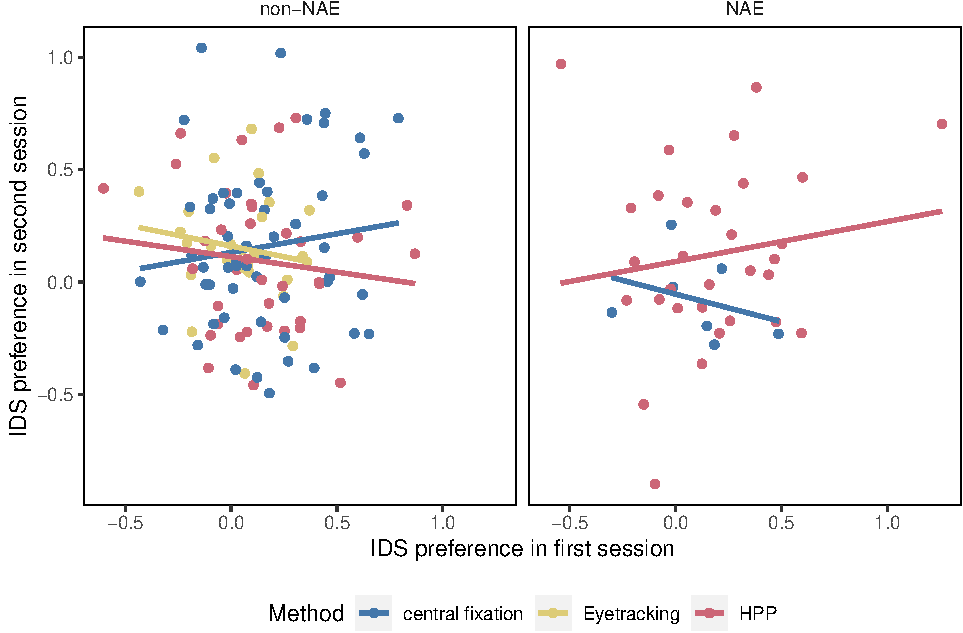
\includegraphics{Retest_current_draft_files/figure-latex/fig1-1.pdf}
\caption{\label{fig:fig1}Infants' preference in Session 1 and Session 2 with individual data points and regression lines color-coded by method (central fixation, eye tracking, or HPP). Results are plotted separately for North American English-learning infants (right panel) and infants learning other languages and dialects (right panel).}
\end{figure}

\hypertarget{results-with-different-inclusion-criteria}{%
\subsection{Results with different inclusion criteria}\label{results-with-different-inclusion-criteria}}

To this point, all analyses were performed on data with the inclusion criteria from MB1. For this, infants needed only 1 out of 8 valid trial pairs to be included in the analyses. Given that the use of more stringent inclusion criteria yielded larger effects sizes within the original MB1 study, we also assessed test-retest reliability by applying stricter inclusion criteria and thereby increasing test length to 2, 4, 6, and 8 non-discard test trials. Applying a stricter criterion and thereby increasing test length, increased descriptively the reliability (Figure 2). In particular, while neither the correlation coefficient based on the inclusion criterion of 2 valid trials, \(t(147) = 0.18\), \(p = .861\), the correlation coefficient based on the inclusion criterion of 4 valid trials, \(t(138) = 0.43\), \(p = .665\), nor the correlation coefficient based on the inclusion criterion of 6 valid trials, \(t(95) = 1.75\), \(p = .084\), were significant, the correlation coefficient based on the inclusion criterion of 8 valid trials - meaning a child had to have no discard trials on both testing days - revealed a significant result, \(t(19) = 2.13\), \(p = .046\). Due to the small sample size and a missing type-1 error correction, we note that this result needs to be treated with caution. Nevertheless, the analyses show that a more stricter inclusion criteria might have led to higher test-retest reliability but at the same time comes with tremendous decreases in sample size.

\begin{figure}

{\centering 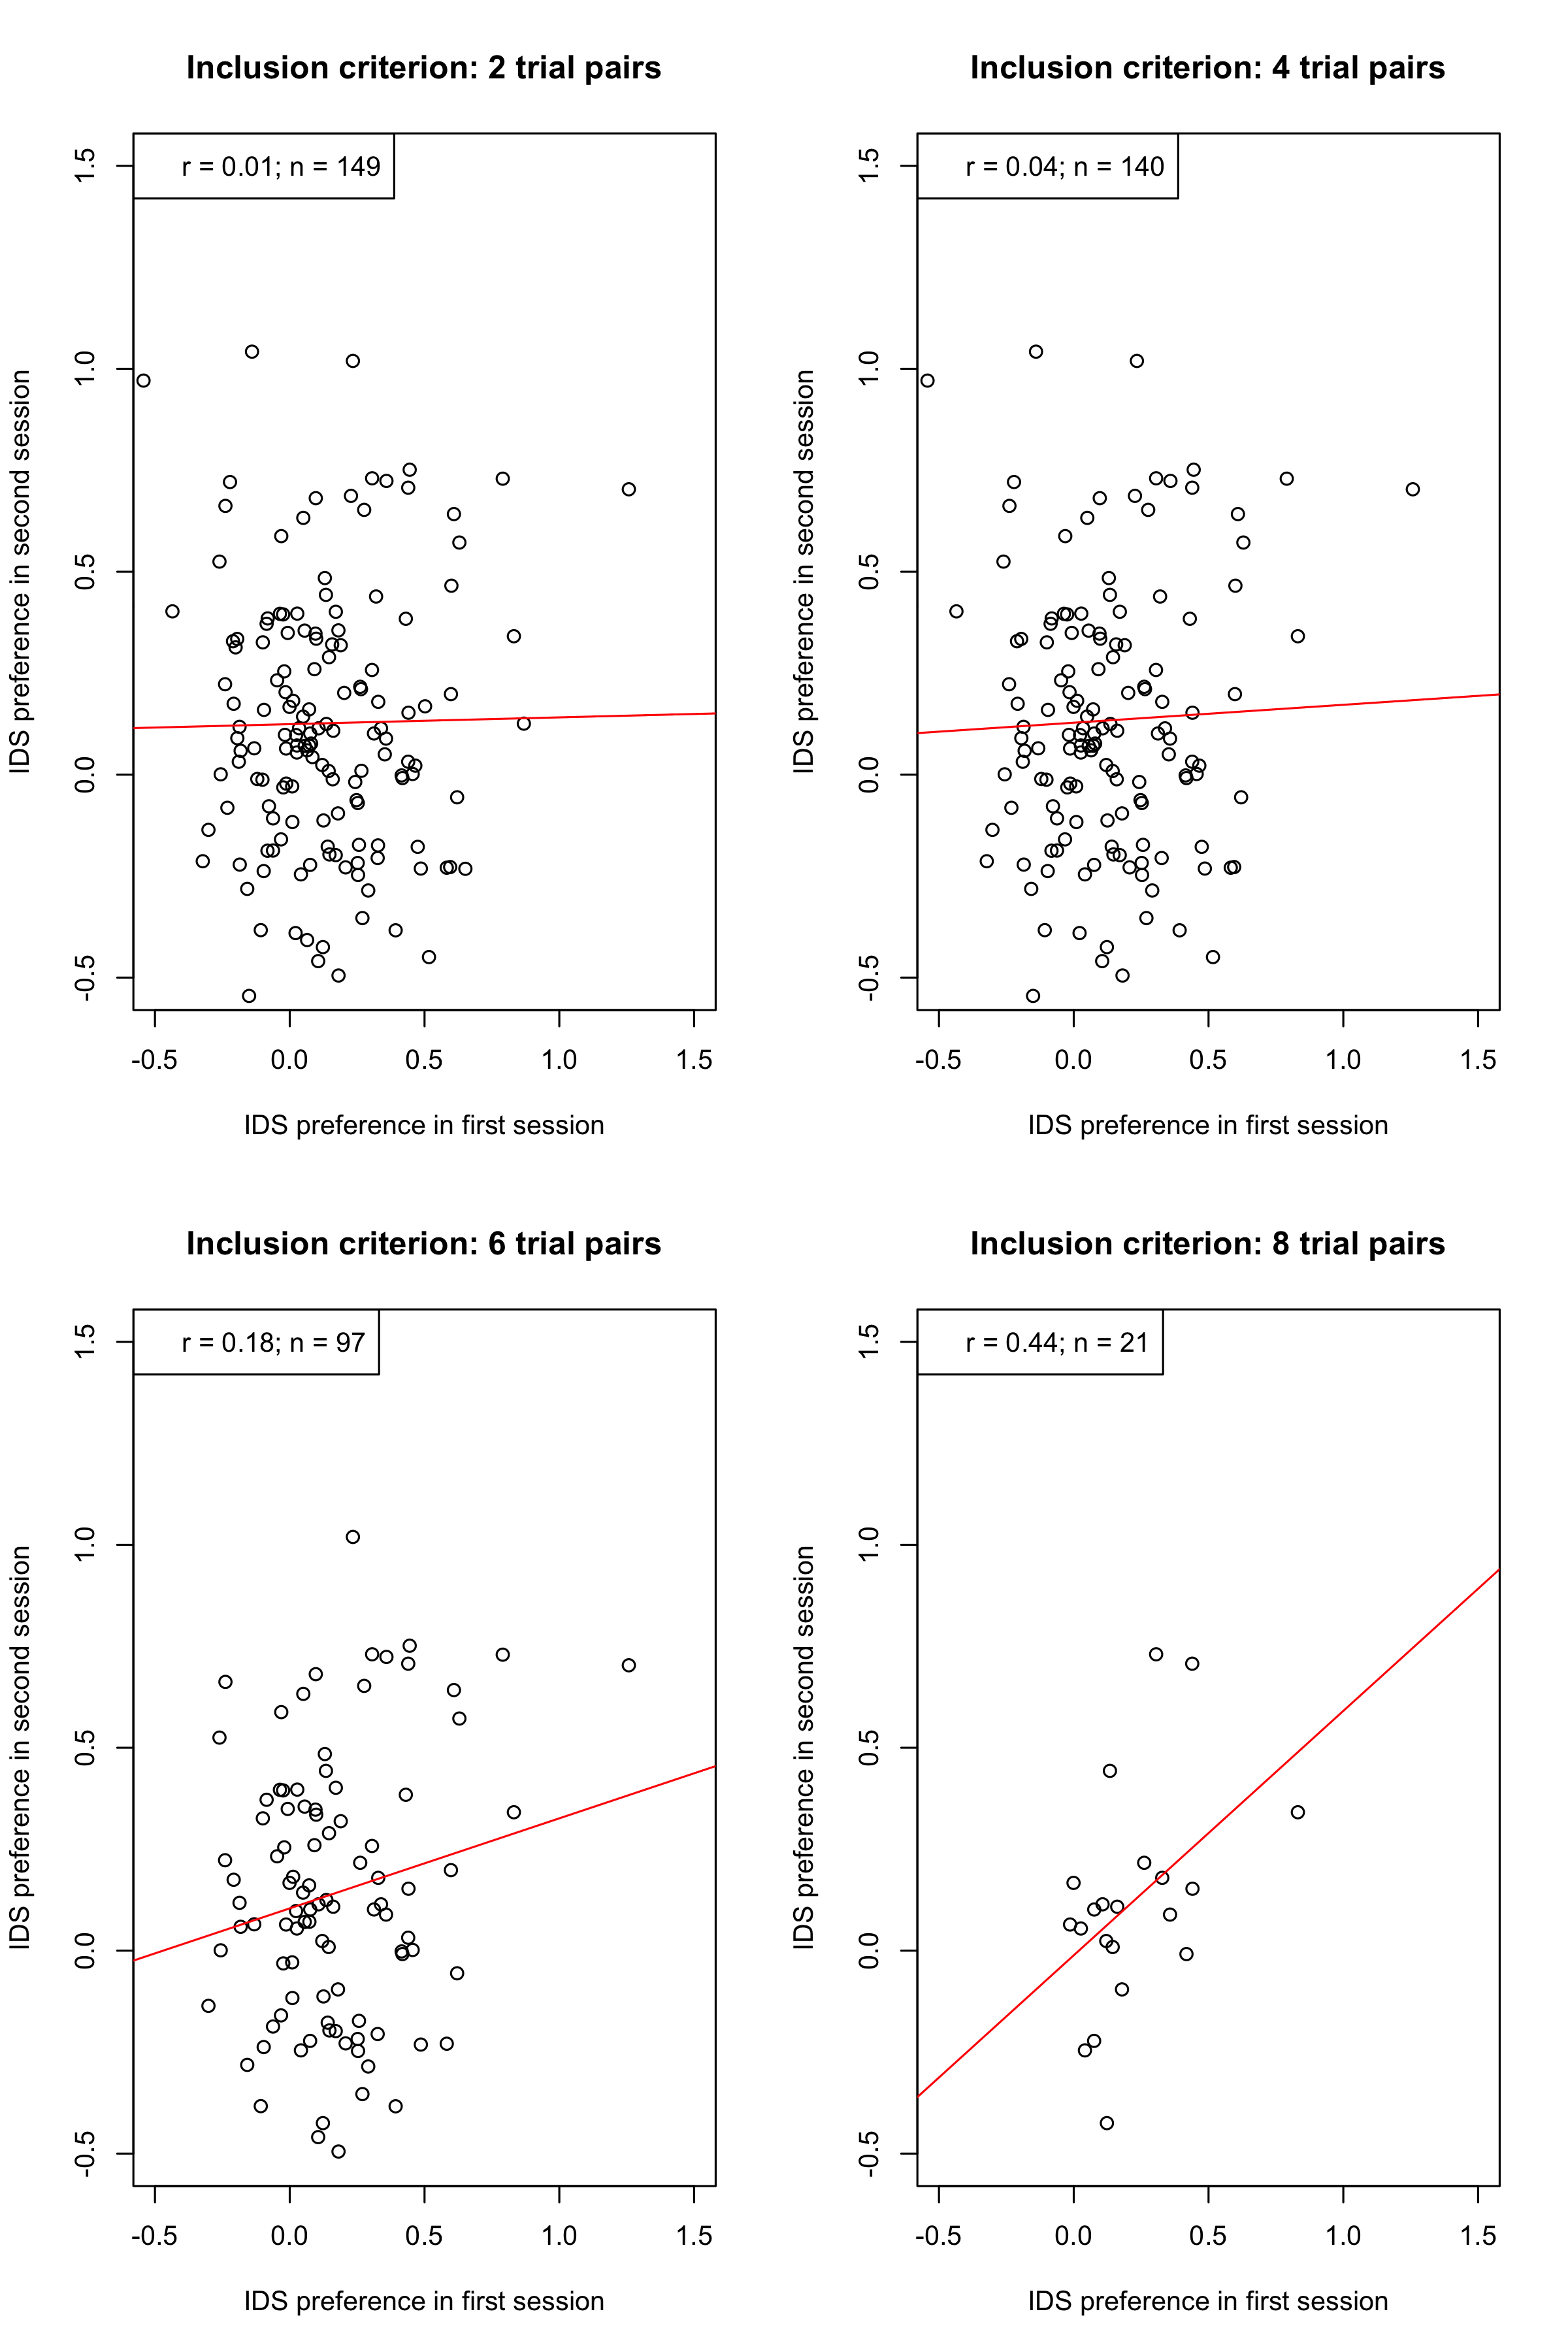
\includegraphics[width=5in]{Retest_current_draft_files/figure-latex/unnamed-chunk-7-1} 

}

\caption{IDS preferences of both sessions plotted against each other for each inclusion criterion. n indicates the number of included infants, r is the Pearson correlation coefficient as the indicator for reliability.}\label{fig:unnamed-chunk-7}
\end{figure}

\hypertarget{general-discussion}{%
\section{General Discussion}\label{general-discussion}}

The current study set out to explore test-retest reliability of infant preference measures which are common experimental paradigms used to study infant cognition. Infants of the original MB1 project were retested on a reversed order of stimuli in order to assess if their listening pattern would be similar to that of their initial assessment. While we replicated the original effect of infants' speech preference for IDS over ADS in the current MB1 follow-up study for both test and retest session using the same MB1 protocol, we did find that infants' speech preference measures had no test-retest reliability. In other words, we were unable to detect any stable individual differences of infants' speech preference. This finding is in line with other research indicating a rather low test-reliability for different developmental paradigms (Cristia et al., 2016). Given that most experimental procedures conducted in developmental research are interested in the comparison of groups, individual differences between participants within a specific condition are usually minimized by the experimental procedure while differences between conditions are maximized. Therefore, infant preference measures may be a good approach to capture universal phenomena but do not seem to be appropriate for examining factors that may lead to differences in development.
Nevertheless, we also detect the effect that increasing test length enhances reliability of the measures, which in turn leads to higher test-retest reliability. A similar effect was found in the MB1 project, where a stricter inclusion criterion led to bigger effect sizes (Consortium, 2020). As in the MB1 original study, higher reliability came at high costs. In particular, due to this strict criterion, only a small portion of the original sample size that is 21 out of 154 infants could be included in the final sample for the analyses. In other words, applying an even stricter criterion leads to an even higher drop out rate and reduces the actual sample sizes enormously. In the case of studies in the field of developmental science, where there are many practical restrictions to collect large samples of infants (e.g., birth rate in the area, restricted lab capacities, budget restrictions), a strict drop out criterion might not be easy - if even possible at all - to implement. Note that studies in developmental science already have above average drop out rates (Miller, 2017).
An alternative approach to increase the number of valid trials might be to also increase the number of collected trials. In this case, a participant can have a high number/proportion of invalid trials and still be included into the final sample as the absolute number of trials is high and thereby decreasing trial-to-trial variability (DeBolt, Rhemtulla, \& Oakes, 2020). While this approach might sound promising, it must be seen if this is realistic, because the attention span of a typical participant of a developmental study is rather short. Therefore, prolonging the experimental procedure to maximize the absolute number of trials might also be practically challenging.
As our results are only based on specific experimental procedure, still with three widely used methods (HPP, central fixation; eye-tracking), developmental studies. need to test the underlining reliability of their measures. Especially, researchers conducting longitudinal studies with experimental data from young infants should be cautious.
One potential explanation for the different behavioral responses to IDS and ADS sequences on the two different testing days may be related to infants' previous experience with laboratory work. As Santolin, Garcia-Castro, Zettersten, Sebastian-Galles, and Saffran (2021) found out, the amount of studies that infants had already participated in may impact their looking patterns with a typical familiarity response for first time visitors moving to preferences of novel items with increasing number of visits.

\hypertarget{limitations}{%
\subsection{Limitations}\label{limitations}}

While we had an above average sample size for a study in developmental research, we were unable to reach the number of participants collected within the original MB1 study. In addition to a delayed call, the extra effort of having to schedule a second lab visit for each participant and the fact that there were already other collaborative studies taking place simultaneously (Byers-Heinlein, Tsui, Bergmann, et al., 2021; Byers-Heinlein, Tsui, Van Renswoude, et al., 2021), might have contributed to the rather low turnout. A higher sample size and a larger number of participating labs from different countries might have enabled us to test for possible differences of the test-retest reliability of the different methods (HPP, central fixation, eye-tracking) and NAE versus non-NAE language backgrounds. Further, a larger sample size might have enabled us to conduct meaningful moderator effects such as age of the child or the effect of native vs.~non-native children on the test-retest reliability.
A further limitation concerns the stimuli. While the order of the stimuli presented to the participating children in the second session was different than in the first session, the exact same stimuli as in MB1 were used in both sessions. In particular, all children heard the exact same voices in Session 1 and in Session 2. From the practical point of view, it was the easiest solution. However, familiarity effects might have played a role for the children. Assuming that only some children might have recognized the voices in Session 2 from their session a week ago, some children might not have done so, for some children a familiarity effect might have happened.

\hypertarget{conclusion}{%
\section{Conclusion}\label{conclusion}}

Following the MB1 protocol, the current study could not detect test-retest reliability of infants' preference measures for IDS over ADS. Subsequent analyses showed that a stricter criterion for the inclusion of data points enhances the test-retest reliability at the cost of high drop out rates. Developmental studies, which rely on stable individual differences of their participants, need to consider the underlying reliability of their measures.

\newpage

\hypertarget{data-and-materials-availability-statement}{%
\section{Data and materials availability statement}\label{data-and-materials-availability-statement}}

The data and materials that support the findings of the current study are openly available on OSF at \url{https://osf.io/ZEQKA/}.

\newpage

\hypertarget{references}{%
\section{References}\label{references}}

\begingroup
\setlength{\parindent}{-0.5in}
\setlength{\leftskip}{0.5in}

\hypertarget{refs}{}
\begin{CSLReferences}{1}{0}
\leavevmode\vadjust pre{\hypertarget{ref-byers2021multilab}{}}%
Byers-Heinlein, K., Tsui, A. S. M., Bergmann, C., Black, A. K., Brown, A., Carbajal, M. J., \ldots{} others. (2021). A multilab study of bilingual infants: Exploring the preference for infant-directed speech. \emph{Advances in Methods and Practices in Psychological Science}, \emph{4}(1), 2515245920974622.

\leavevmode\vadjust pre{\hypertarget{ref-byers2021development}{}}%
Byers-Heinlein, K., Tsui, R. K.-Y., Van Renswoude, D., Black, A. K., Barr, R., Brown, A., \ldots{} others. (2021). The development of gaze following in monolingual and bilingual infants: A multi-laboratory study. \emph{Infancy}, \emph{26}(1), 4--38.

\leavevmode\vadjust pre{\hypertarget{ref-colombo1988infant}{}}%
Colombo, J., Mitchell, D. W., \& Horowitz, F. D. (1988). Infant visual attention in the paired-comparison paradigm: Test-retest and attention-performance relations. \emph{Child Development}, 1198--1210.

\leavevmode\vadjust pre{\hypertarget{ref-manybabies2020quantifying}{}}%
Consortium, M. (2020). Quantifying sources of variability in infancy research using the infant-directed-speech preference. \emph{Advances in Methods and Practices in Psychological Science}, \emph{3}(1), 24--52.

\leavevmode\vadjust pre{\hypertarget{ref-cooper1990preference}{}}%
Cooper, R. P., \& Aslin, R. N. (1990). Preference for infant-directed speech in the first month after birth. \emph{Child Development}, \emph{61}(5), 1584--1595.

\leavevmode\vadjust pre{\hypertarget{ref-cristia2016test}{}}%
Cristia, A., Seidl, A., Singh, L., \& Houston, D. (2016). Test--retest reliability in infant speech perception tasks. \emph{Infancy}, \emph{21}(5), 648--667.

\leavevmode\vadjust pre{\hypertarget{ref-debolt2020robust}{}}%
DeBolt, M. C., Rhemtulla, M., \& Oakes, L. M. (2020). Robust data and power in infant research: A case study of the effect of number of infants and number of trials in visual preference procedures. \emph{Infancy}, \emph{25}(4), 393--419.

\leavevmode\vadjust pre{\hypertarget{ref-frank2017collaborative}{}}%
Frank, M. C., Bergelson, E., Bergmann, C., Cristia, A., Floccia, C., Gervain, J., \ldots{} Yurovsky, D. (2017). A collaborative approach to infant research: Promoting reproducibility, best practices, and theory-building. \emph{Infancy}, \emph{22}(4), 421--435. \url{https://doi.org/10.1111/infa.12182}

\leavevmode\vadjust pre{\hypertarget{ref-hedge2018reliability}{}}%
Hedge, C., Powell, G., \& Sumner, P. (2018). The reliability paradox: Why robust cognitive tasks do not produce reliable individual differences. \emph{Behavior Research Methods}, \emph{50}(3), 1166--1186.

\leavevmode\vadjust pre{\hypertarget{ref-houston2007assessing}{}}%
Houston, D. M., Horn, D. L., Qi, R., Ting, J. Y., \& Gao, S. (2007). Assessing speech discrimination in individual infants. \emph{Infancy}, \emph{12}(2), 119--145.

\leavevmode\vadjust pre{\hypertarget{ref-klein2014}{}}%
Klein, R. A., Ratliff, K. A., Vianello, M., Adams Jr, R. B., Bahník, Š., Bernstein, M. J., \ldots{} Nosek, B. A. (2014). Investigating variation in replicability. \emph{Social Psychology}, \emph{45}, 142--152. \url{https://doi.org/10.1027/1864-9335/a000178}

\leavevmode\vadjust pre{\hypertarget{ref-miller2017developmental}{}}%
Miller, S. A. (2017). \emph{Developmental research methods}. Sage publications.

\leavevmode\vadjust pre{\hypertarget{ref-open2015estimating}{}}%
Open Science Collaboration. (2015). Estimating the reproducibility of psychological science. \emph{Science}, \emph{349}(6251), aac4716. \url{https://doi.org/10.1126/science.aac4716}

\leavevmode\vadjust pre{\hypertarget{ref-santolin2021experience}{}}%
Santolin, C., Garcia-Castro, G., Zettersten, M., Sebastian-Galles, N., \& Saffran, J. R. (2021). Experience with research paradigms relates to infants' direction of preference. \emph{Infancy}, \emph{26}(1), 39--46.

\end{CSLReferences}

\endgroup


\end{document}
